\documentclass[french, 12pt]{article}%


\usepackage[T1]{fontenc}
\usepackage[utf8]{inputenc}
\usepackage[french]{babel}

\usepackage{textcomp}

\usepackage[official]{eurosym}

\usepackage{appendix}
\usepackage{pdfpages}

%%%%%%%%%%%%%%%%%%%%%%%%%%%%%%%%%%%%%%%%%%%%%%%%%%%%%%%%%
\newcommand{\itemE}{\item[$\bullet$]}

\newcommand{\titreSeq}{Gestion des logs}
\newcommand{\lycee}{Académie rennes}
\newcommand{\classSeq}{CIEL }
\newcommand{\matiereSeq}{IR}      
\newcommand{\numSeq}{Cyber}
\newcommand{\numAct}{05}
\newcommand{\objSeance}{Comment gérer les logs}

\newcommand{\moySeq}{\begin{itemize}	
\itemE VM Kali
\itemE VM serveurCyber
\itemE VM Pfsense
\end{itemize}}


\newcommand{\paraL}[1]{\tiny\noindent\rule{1.0\linewidth}{0.5pt}\paragraph*{#1}\  \normalsize}


\newcommand{\compSeq}{\begin{itemize}
\item  
\end{itemize}}
%%%%%%%%%%%%%%%%%%%%%%%%%%%%%%%%%%%%%%%%%%%%%%%%%%%%%%%%%%

%%%%%%%%%%%%%%%%%%%%%%%%%%%%%%%%%%%%%%%%%%%%%%%%%%%%%%%%
%%%%Algo
\usepackage[linesnumbered, french]{algorithm2e}
\SetKwFor{For}{Pour}{faire}{fin}
\SetKwFor{While}{Tant que}{faire}{fin}%
\SetKw{KwTo}{?}
\SetKw{KwPas}{par pas de}
\SetKw{KwRet}{Retourne}
\SetKwProg{Fn}{Fonction }{ arguments }{fin}
\SetKwRepeat{Repeat}{Répéter}{jusqu'?}%
\SetKwIF{If}{ElseIf}{Else}{Si}{alors}{Sinon si}{Sinon}{Fin}


\usepackage{listings} %%%%Présenration code source
\lstset{language=C++,
    %numbers=left,
   %stepnumber=1,
    showstringspaces=false,
    tabsize=1,
    breaklines=true,
    breakatwhitespace=false,
    basicstyle=\footnotesize,
    keywordstyle=\color{blue}\footnotesize,
    stringstyle=\color{red}\footnotesize,
    commentstyle=\color{magenta}\footnotesize,
    morecomment=[l][\color{magenta}]{\#}
    }
\lstdefinestyle{commande}{
  basicstyle=\ttfamily\footnotesize,
  keywordstyle=\color{blue},
  commentstyle=\color{gray},
  %numbers=left,
  %numberstyle=\tiny\color{gray},
  numbersep=5pt,
  breaklines=true,
  frame=single,
  backgroundcolor=\color{lightgray!10},
  %captionpos=b,
  %caption=\lstname   
    extendedchars=true,
    literate={é}{{\'e}}1
             {è}{{\`e}}1
             {à}{{\`a}}1
             {ç}{{\c{c}}}1
             {✔}{{\checkmark}}1,
}
%\usepackage[T1]{fontenc}

\newcommand{\itemB}{\item[$\Box$]}
% Margins
\topmargin=-0.45in
\evensidemargin=0in
\oddsidemargin=0in
\textwidth=6.5in
\textheight=9.0in
\headsep=0.25in 
\usepackage{multicol}

\linespread{1.1} 
\usepackage{amsmath}%
\usepackage{amsfonts}%
\usepackage{amssymb}%
\usepackage{graphicx}
\usepackage{lastpage}
\usepackage{enumitem}

%\usepackage[T1]{fontenc}    
\usepackage{multirow}
\usepackage{lscape}
\usepackage[colorlinks = true,
            linkcolor = blue,
            urlcolor  = blue,
            citecolor = blue,
            anchorcolor = blue]{hyperref}
\usepackage{array}
\usepackage{mwe}
%-------------------------------------------
\newtheorem{theorem}{Theorem}
\newtheorem{summary}[theorem]{Summary}
\newenvironment{proof}[1][Proof]{\textbf{#1.} }{\ \rule{0.5em}{0.5em}}



\usepackage{xcolor}

\usepackage{colortbl}
\definecolor{vert_capet}{RGB}{191,255,191}	
\definecolor{bleu_snir}{RGB}{101,191,179}	
\setlength{\doublerulesep}{\arrayrulewidth}
%-------------------------------------------
%%%%%%%%%%%%%%%%%%%%%%%%%%%%%%%%%%%%%%%%%%%%%
\usepackage[framemethod=tikz]{mdframed}
\usepackage{tikz, xcolor, lipsum}
\makeatletter
\mdfsetup{skipabove=\topskip,skipbelow=\topskip}

\tikzset{titre_bleu_snir/.style =
	{draw=bleu_snir, line width=1.5pt, fill=white,
	rectangle, rounded corners, right,minimum height=2em}}
\newcommand{\titreencadre}{Titre}
\makeatletter
\mdfdefinestyle{encadrestyle}{%
	linewidth=1.5pt,roundcorner=5pt,linecolor=bleu_snir,
	apptotikzsetting={\tikzset{mdfbackground/.append style ={%
		fill=white}}},
	frametitlefont=\bfseries,
	singleextra={%
		\node[titre_bleu_snir,xshift=2em] at (P-|O) %
			{~\mdf@frametitlefont{\titreencadre}\hbox{~}};},
	firstextra={%
		\node[titre_bleu_snir,xshift=2em] at (P-|O) %
		{~\mdf@frametitlefont{\titreencadre}\hbox{~}};},
	}
\mdfdefinestyle{encadresanstitrestyle}{%
	linewidth=1.5pt,roundcorner=5pt,linecolor=bleu_snir
	apptotikzsetting={\tikzset{mdfbackground/.append style ={%
		fill=yellow!20}}},
	}

\newenvironment{encadre}[1]{\renewcommand{\titreencadre}{#1}
	\begin{mdframed}[style=encadrestyle]
	\vspace{0.5\baselineskip}
	}{%
	\end{mdframed}}

\newenvironment{encadresanstitre}{
	\begin{mdframed}[style=encadresanstitrestyle]
	}{%
	\end{mdframed}}
\makeatother
\usepackage{colortbl}
\definecolor{vert_capet}{RGB}{191,255,191}	
\definecolor{bleu_snir}{RGB}{101,191,179}	
\setlength{\doublerulesep}{\arrayrulewidth}
%-------------------------------------------
\usepackage{comment}
%%%%%%%%%%%%%%%%%%%%%%%%%%%%%%%
\newif\ifPROF

%\def\PourProf{0}
\ifdefined\PourProf
  \PROFtrue
  \newenvironment{corr}{\begingroup \color{red}}{\normalcolor \endgroup}
\else
  \PROFfalse
  \newenvironment{corr}{\begingroup \color{white}}{\normalcolor \endgroup}
\fi

%\PROFtrue

%%%%%%%%%%%%%%%%%%%%%%%%%%%%%%%%%%%%




%%%Note et pied de page
\usepackage{fancybox}
\usepackage{fancyhdr}
\usepackage[a4paper,margin=2.5cm,bottom=2cm,headheight=2cm]{geometry}
\pagestyle{fancy}
\fancyhead[R]{
\includegraphics[scale=0.3]{logo_CIEL.png}}
\fancyhead[C]{Prénom}
\fancyhead[L]{Nom}
\fancyfoot[C]{Page \thepage/\pageref{LastPage}}
\fancyfoot[L]{\classSeq ~\matiereSeq}
\fancyfoot[R]{Formation \numSeq  ~ Act \numAct}
\renewcommand{\headrulewidth}{1pt}
%%%Note et pied de page 



\begin{document}
\lstset{basicstyle = \ttfamily,columns=fullflexible}

\title{\titreSeq\\
 \includegraphics[scale=0.5]{logo_sti2d.png}\\
}
\author{\lycee}
\date{}%\today}
%\maketitle

\noindent\begin{tabular}{!{\vrule width 1.5pt}m{0.7\linewidth}!{\vrule width 1.5pt}m{0.2\linewidth}!{\vrule width 1.5pt}}
\hline\hline
\cellcolor{green!25}
\begin{center}
	\Large\textbf{\titreSeq}  
\end{center}
  & 

\begin{minipage}{1.0\linewidth}
  \vspace*{0.1cm} 
\centering
\includegraphics[scale=0.2]{logo_lycee.jpg}

{\tiny\today}
  \vspace*{0.1cm} 
\end{minipage}\\ \hline\hline

\multicolumn{2}{!{\vrule width 1.5pt}l!{\vrule width 1.5pt}}{
\begin{minipage}{14cm}
\vspace*{0.1cm} 
\textbf{Objectif} : \objSeance
\vspace*{0.1cm} 
\end{minipage}} \\ \hline\hline

\multicolumn{2}{!{\vrule width 1.5pt}l!{\vrule width 1.5pt}}{
\begin{minipage}{14cm}
\vspace*{0.1cm} 
\textbf{Moyens} : 
\moySeq
\vspace*{0.1cm} 
\end{minipage}} \\ \hline\hline
%
%\multicolumn{2}{!{\vrule width 1.5pt}l!{\vrule width 1.5pt}}{
%\begin{minipage}{14cm}
%\vspace*{0.1cm}
%\tiny
%Compétences attendues :
%\compSeq
%\vspace*{0.1cm}
%\end{minipage}}
%\normalsize \\ \hline\hline
\end{tabular}

\tableofcontents
\newpage


%%%%%%%%%%%%%%%%%%%%%%%%%%%%%%%%%%%%%%%%%%%%%%%%%%%%%%%%%%%%%%%%%%%%%%%%%%%%%%%%
%%%%%%%%%%%%%%%%%%%%%%%%%%%%%%%%%%%%%%%%%%%%%%%%%%%%%%%%%%%%%%%%%%%%%%%%%%%%%%%
\section{Les logs}

\begin{encadre}{Log}
Enregistrement chronologique d'événements, d'actions ou de messages générés par un système informatique, utilisé pour le suivi, le diagnostic et la sécurité.
\end{encadre}

Dans cette activité, nous allons voir un moyen pour centraliser les logs. 


La centralisation des logs est très importante pour la supervision des systèmes  et présente de nombreux avantages 
\begin{itemize}
\itemE Facilité l'analyse globale des logs
\itemE Retracer l'origine de problème
\itemE Identifie des incidents complexes en croisant les logs de différentes sources 
\itemE Détection automatique d’anomalies ou d’erreurs critiques grâce à des règles d’alerte sur les logs.

\end{itemize}

\section{Principe générale}
De la même manière que pour Prometheus, la centralisation des logs va être mise en place à l'aide de 3 containers 
\begin{itemize}
\itemE \textbf{Promtail} : agent (ou service) qui collecte les logs sur un système Promtail pour \textit{Tailing logs in Prometheus format}
\itemE  \textbf{Grafana} : Outil de mise en page des données (que l'on ne représente plus)
\itemE  \textbf{Loki} : outils de centralisation des données.
\end{itemize}

\begin{center}
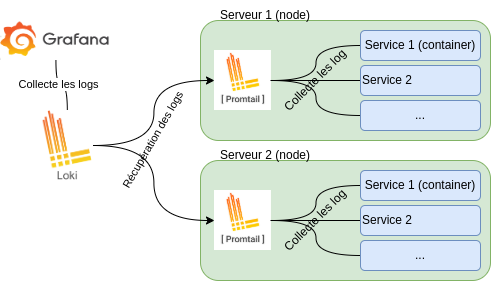
\includegraphics[scale=0.7]{./ressource/loki_Protmail.png}
\end{center}


\section{Pré-requis}
Pour effectuer le test de logs dans les meilleurs conditions, il est nécessaire de stopper les containers des tests précédents. Pour cela, soit vous allez dans \textbf{tous les répertoires} contenant vos \verb?docker-compsoe.yml? et vous taper la commande 
\begin{lstlisting}[style=commande]
sudo docker compose down
\end{lstlisting}

Soit vous taper juste suivante/ Elle arrête tous les containers \textbf{Attention si vous en avez d'autres qui ne doivent pas être arrêtes}.
\begin{lstlisting}[style=commande]
sudo docker stop $(sudo docker ps -q)
\end{lstlisting}

Normalement la commande pour visualiser les container lancés ne retourne rien

\begin{lstlisting}[style=commande]
$ sudo docker ps
CONTAINER ID   IMAGE     COMMAND   CREATED   STATUS    PORTS     NAMES
\end{lstlisting}


\paragraph{Service à scruter} \

Pour les tests, les logs des \textbf{services LEMP en HTTP} (non sécurisé) vont être collectés. Il est donc ncéessaire de le relancer. 
Pour rappel : 
\begin{itemize}
\itemE L'URL du dépôt est  : \url{https://github.com/PierreViland/00-serveurLemp.git}
\itemE La branche a utilisé est : \verb?main?
\begin{lstlisting}[style=commande]
$ git switch main
Already on 'main'
Your branch is up to date with 'origin/main'.
\end{lstlisting}

\itemE La commande pour l'ensemble l'ensemble des containers est : 
\begin{lstlisting}[style=commande]
$ sudo docker compose up -d
\end{lstlisting}


\end{itemize} 

\section{Mise en place de Promtail}

L'ensemble des éléments de configuration de la centralisation des logs est présente sur \textbf{ le même dépôt que Prometheus} 
\begin{itemize}
\itemE \url{https://github.com/PierreViland/reverseProxyMonitoringPV.git}
\end{itemize}

Le lancement d'un container Promtail doit se faire sur chaque serveur. Les lignes du fichier \verb?docker-compose.yml? sont les suivantes : 

\begin{lstlisting}[style=commande]
 55   promtail:
 56     image: grafana/promtail:latest
 57     container_name: promtail
 58     volumes:
 59       - /var/log:/var/log
 60       - /var/lib/docker/containers:/var/lib/docker/containers:ro        
 61       - ./promtail-config.yaml:/etc/promtail/config.yaml
\end{lstlisting}
avec : 
\begin{itemize}
\itemE \verb? - /var/log:/var/log? : volume partagé contant les logs de la machines hôte. \textbf{A modifier sous windows}
\itemE \verb? - /var/lib/docker/containers:/var/lib/docker/containers:ro   ? : volume partagé contenant les fichiers des containers
\itemE \verb?- ./promtail-config.yaml:/etc/promtail/config.yaml?  : fichier de configuration de promtail
\end{itemize}



Le fichier de configuration de promtail se nomme \verb?promtail-config.yaml?. Il contient les éléments suivants qui peuvent être bien sûr modifier en fonction des besoins?

\begin{lstlisting}[style=commande]

\end{lstlisting}


\begin{lstlisting}[style=commande]
server:
  http_listen_port: 9080
  grpc_listen_port: 0
\end{lstlisting}
avec : 
\begin{itemize}
\itemE  \verb? http_listen_port: 9080? : Promtail écoute sur le port 9080 pour l'interface HTTP.
\itemE  \verb?grpc_listen_port: 0? : Le port gRPC (Remote Procedure Call) est désactivé (valeur 0).
\end{itemize}

Ensuite on retrouve 
\begin{lstlisting}[style=commande]
clients:
  - url: http://loki:3100/loki/api/v1/push
\end{lstlisting}
qui spécifie où envoyer les logs. \verb?loki? est le nom du container (qui peut aussi être l'adresse IP) suivi de son port d'écoute \verb?3100?. Le reste de l'URL \verb?/loki/api/v1/push? ne peut pas être modifié.


Ensuite, il est précisé le nom du fichier utilisé pour suivre la position de lecture des logs (évite de tout relire à chaque démarrage).
\begin{lstlisting}[style=commande]
positions:
  filename: /tmp/positions.yaml
\end{lstlisting}
\textbf{A modifier sous Windows}




C'est ensuite que les différents \textbf{jobs} sont configuré permettant de dire à Promtail qu'elle logs nous devons récupérer. 

\begin{lstlisting}[style=commande]
scrape_configs:
\end{lstlisting}

Dans cette exemple, le premier job récupère les logs du système hôte. \textbf{A modifier sous Windows}
\begin{lstlisting}[style=commande]
  # Scrap tous les log de mon hote
  - job_name: system
    static_configs:
      - targets:
          - localhost
        labels:
          job: varlogs
          __path__: /var/log/*.log
\end{lstlisting}

Ensuite, il est configuré la récupération des logs du container nginx  ayant pour ID \textbf{8526.....022d}. 
\begin{lstlisting}[style=commande]
- job_name: nginx_container

    static_configs:
      - targets:
          - localhost
        labels:
          job: nginx
          container: nginxPV
          __path__: /var/lib/docker/containers/85268aa8e6cb59dd445a21d3796339e345f641f6e3e91b7606b7d495c342022d/85268aa8e6cb59dd445a21d3796339e345f641f6e3e91b7606b7d495c342022d-json.log
\end{lstlisting}
La strucutre est similaire à la récupération des logs système : 
\begin{itemize}
\itemE \verb?target ? : représente le points de collecte.
\itemE \verb?job: nginx? : nom du job (qui sera utilisé par loki)
\itemE \verb?container: nginxPV ? : identifie le conteneurs 
\itemE \verb?__path__ ? : chemin exact du fichier de logs du conteneur.
\end{itemize}

La suite des lignes est toujours relative au job \verb?nginx_container?. On y retrouve les \textbf{pipeline\_stages} qui sont des étapes de traitements des logs avant d'envoyer à loki. 


\begin{lstlisting}[style=commande]
    pipeline_stages:    
      - json:
          expressions:
            log: log 

      - regex:
          expression: '"(?P<method>[A-Z]+)'

\end{lstlisting}

La première étape consiste à récupérer la clef "log" de l'objet JSON. 
\begin{lstlisting}[style=commande]
      - json:
          expressions:
            log: log 
\end{lstlisting}


La 2e étape consiste à appliquer une expression régulière sur la chaine \verb?log? extraite précédemment. 
\begin{lstlisting}[style=commande]
- regex:
    expression: '"(?P<method>[A-Z]+)'
\end{lstlisting}
\begin{itemize}
\itemE Recherche \verb?"?
\itemE Le texte capture sera accessible sous le nom method
\itemE On doit retrouver une ou plusieurs majuscule dans le texte recherché. Li'dée est de trouver les méthode HTTPS, GET, POST,...
\end{itemize}
Les IA type chatGPT sont très performantes pour générer des expressions régulières. Il ne faut pas s'en priver. Il est possible dans ce cas d'optimiser la recherche en remplaçant la regex par : 

\verb?(P<method>GET|POST|PUT|DELETE|PATCH|OPTIONS|HEAD)? où l'on précise explicitement les méthodes HTTP. 



La 3e étape prend la valeur extraite précédemment (\verb?method?) et l'ajoute comme label Loki.
\begin{lstlisting}[style=commande]
      - labels:
          method:
\end{lstlisting}



Comme nous le verrons dans la suite du document, les labels permettent des rechercher efficacement dans \textbf{loki}. Attention cependant à ne pas trop en abuser sans quoi les performances de loki seront impactées. 

\section{Mise en place de loki}

Pou rappel, \textbf{Loki} permet la centralisation des données. Les lignes du \verb?docker-compose.yml? relatives à sont lancement sont : 
\begin{lstlisting}[style=commande]
 41   loki:
 42     image: grafana/loki:latest
 43     container_name: loki
 44     ports:
 45       - "3100:3100"
 46     command:
 47       - "-config.file=/etc/loki/local-config.yaml"
 48     volumes:
 49       - ./loki-config.yaml:/etc/loki/local-config.yaml
 50       - ./loki-data:/data       
 51     user: "1000:1000"
 52     networks:
 53       - mynet
\end{lstlisting}


Le fichier de configuration est présent dans le dépôt et se nomme \verb?loki-config.yaml?. Aucune modification de ce fichier est nécessaire pour faire fonctionner loki. Il faut juste bien vérifier que le port d'écoute de loki soit le 3100
pour être en accord avec la configuration de promtail.
\begin{lstlisting}[style=commande]
server:
  http_listen_port: 3100
\end{lstlisting}



\section{Grafana}

\paragraph{Connexion avec loki}
\textbf{Grafana}, outil déjà utilisé va permette de visualiser les logs. la première étape de de créer \textbf{une connexion de Grafana a Loki}. 

\begin{center}
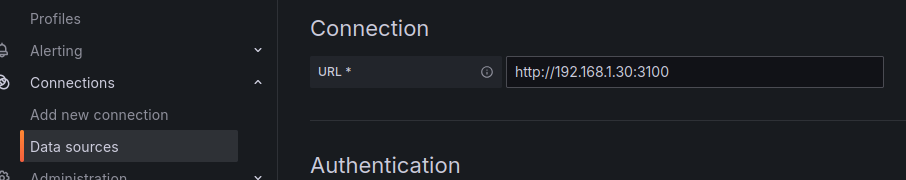
\includegraphics[scale=0.7]{./ressource/grafanRef_loki}
\end{center}
Dans le cas détaillé dans l'image ci-dessous, les logs sont récupérés via un container loki installé sur la machine \verb?192.168.1.30? en écoute sur le port \verb?3100?.


\paragraph{Explorer}


L'onglet Explore est une interface qui permet de consulter et analyser les logs en temps réel. Il est par exemple très facile de lister les log correspondant à une méthode GET ou une méthode POST. 
\begin{center}
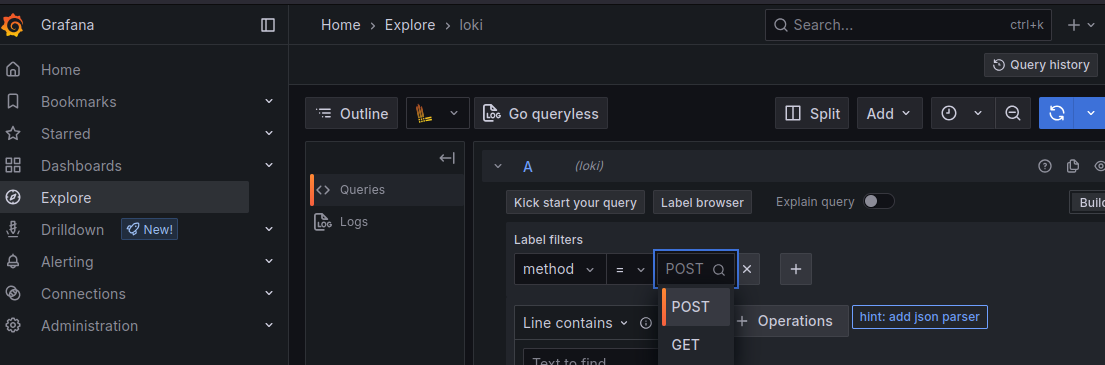
\includegraphics[scale=0.5]{./ressource/grafanaExplore}
\end{center}


\paragraph{Modification du dashbord}
Il est aussi possible de rajouter dans un dashbord le nombre de connexion GET (ou POST par minute : 
\begin{lstlisting}[style=commande]
sum(count_over_time({job="nginx", method="GET"}[1m]))
\end{lstlisting}
\begin{center}
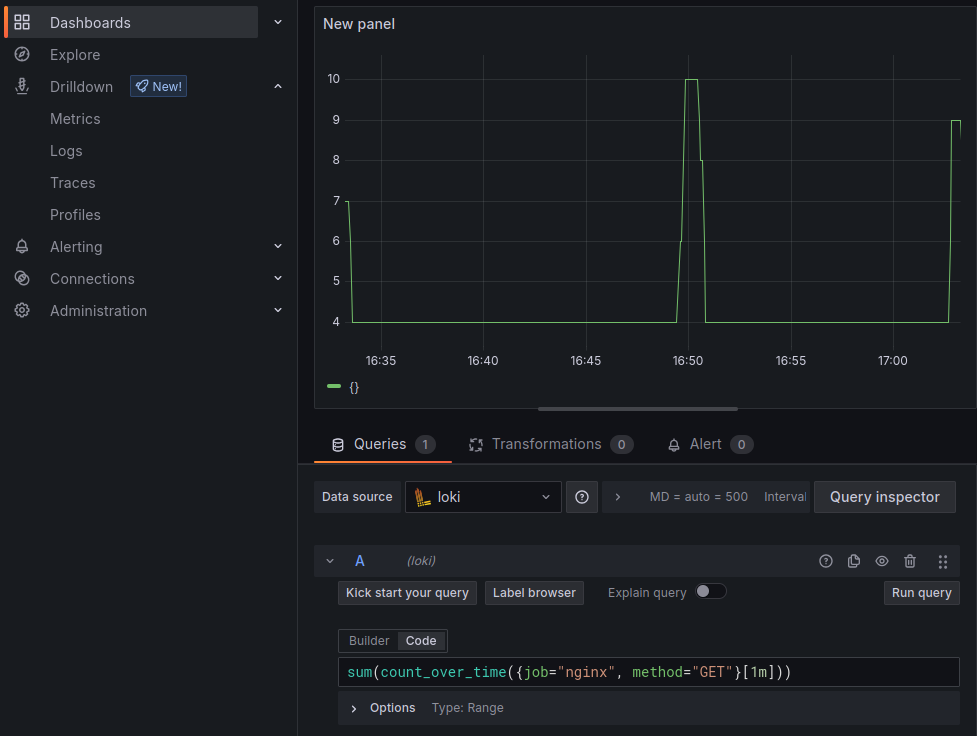
\includegraphics[scale=0.5]{./ressource/grafanaNombre_delelement.png}
\end{center}

\end{document}